\documentclass[10pt]{beamer}
\usepackage[utf8]{inputenc}
\usepackage[francais]{babel}
\usepackage[T1]{fontenc}
\usepackage[export]{adjustbox}
\newcommand\Fontvi{\fontsize{8}{7.2}\selectfont}
\usepackage{tabularx}
\usepackage{minted}
\usemintedstyle{colorful}
\definecolor{mygray}{gray}{0.95}
\newenvironment{code}{\captionsetup{type=listing}}{}

\usepackage{hyperref}
\hypersetup{
    colorlinks,
    citecolor=black,
    filecolor=black,
    linkcolor=black,
    urlcolor=blue
}

\usetheme{Frankfurt}
\usecolortheme{beaver}

\addtobeamertemplate{navigation symbols}{}{%
    \usebeamerfont{footline}%
    \usebeamercolor[fg]{footline}%
    \hspace{1em}%
    \insertframenumber/\inserttotalframenumber
}

\titlegraphic{
\includegraphics[width=0.5\textwidth]{images/title.png}}

\begin{document}
\logo{%
    \makebox[0.95\paperwidth]{%
        
\includegraphics[width=2.5cm,keepaspectratio]{images/hepia.jpg}%
        \hfill%
        
\includegraphics[width=2.5cm,keepaspectratio]{images/hesso.jpg}%
    }%
}

\title{TagFS - Système d'étiquetage des fichiers avec Rust}
\author{Steven Liatti}
\institute{Projet de bachelor - Prof. Florent Glück - Hepia ITI 3\up{ème} année}
\date{4 septembre 2018}

\begin{frame}
\titlepage
\end{frame}

\begin{frame}
    \frametitle{Plan}
    \setcounter{tocdepth}{1}
    \tableofcontents
\end{frame}

%%%%%%%%%%%%%%%%%%%%%%%%%%%%%%%%%%%%%%%%%%%%%%%%%%%%%%%%%%%%%%%%%%%%%%%%%%%%%%%%%%%%%%%%%%%%%%%%%%%
%%%%%%%%%%%%%%%%%%%%%%%%%%%%%%%%%%%%%%%%%%%%%%%%%%%%%%%%%%%%%%%%%%%%%%%%%%%%%%%%%%%%%%%%%%%%%%%%%%%
\section{Introduction}
\subsection{Problématique}
\begin{frame}
    \frametitle{\subsecname}
    \begin{itemize}
        \item Nombre de fichiers énorme.
        \pause
        \item Difficulté à retrouver des fichiers.
        \pause
        \item Plusieurs emplacements logiques pour un seul fichier.
        \pause
    \end{itemize}
    \Large\textbf{Système de tags de fichiers et répertoires avec possibilité de recherche par tags.}
\end{frame}

\subsection{Objectifs}
\begin{frame}
    \frametitle{\subsecname}
    \begin{itemize}
        \item Étudier et s'approprier le langage Rust.
        \pause
        \item Répertorier les applications existantes permettant d'étiqueter les fichiers.
        \pause
        \item Étudier les XATTR lors des manipulation courantes sur les fichiers.
        \pause
        \item Explorer les méthodes de surveillance du système de fichiers.
        \pause
        \item Analyser les moyens d'indexer une arborescence de fichiers.
        \pause
        \item Concevoir et implémenter un système performant.
        \pause
        \item Mesurer les performances de ce système.
    \end{itemize}
\end{frame}

%%%%%%%%%%%%%%%%%%%%%%%%%%%%%%%%%%%%%%%%%%%%%%%%%%%%%%%%%%%%%%%%%%%%%%%%%%%%%%%%%%%%%%%%%%%%%%%%%%%
%%%%%%%%%%%%%%%%%%%%%%%%%%%%%%%%%%%%%%%%%%%%%%%%%%%%%%%%%%%%%%%%%%%%%%%%%%%%%%%%%%%%%%%%%%%%%%%%%%%
\section{Solutions existantes}
\subsection{TMSU et Tagsistant}
\begin{frame}
    \frametitle{\subsecname}
    \begin{itemize}
        \item CLI.
        \item Gestion des tags.
        \item Liste des fichiers associés à des tags.
        \item Usage de commandes usuelles (\mintinline{bash}{cp}, \mintinline{bash}{ls}, 
            \mintinline{bash}{mkdir}) pour manipuler les tags (Tagsistant).
    \end{itemize}
    \pause
    \begin{center}
        \begin{tabularx}{8cm}{|X|X|} \hline
            \textbf{Points positifs} & \textbf{Points négatifs} \\ \hline
            Simple (CLI) & Dépendance à FUSE \\ \hline
            Rapide et efficace & Dépendance à une BDD externe \\ \hline
            Open source & Modification et accès uniquement par l'application (Tagsistant) \\ \hline
        \end{tabularx}
    \end{center}
\end{frame}

\subsection{TagSpaces}
\begin{frame}
    \frametitle{\subsecname}
    \begin{columns}[T]
        \begin{column}{.6\textwidth}
            \begin{figure}
                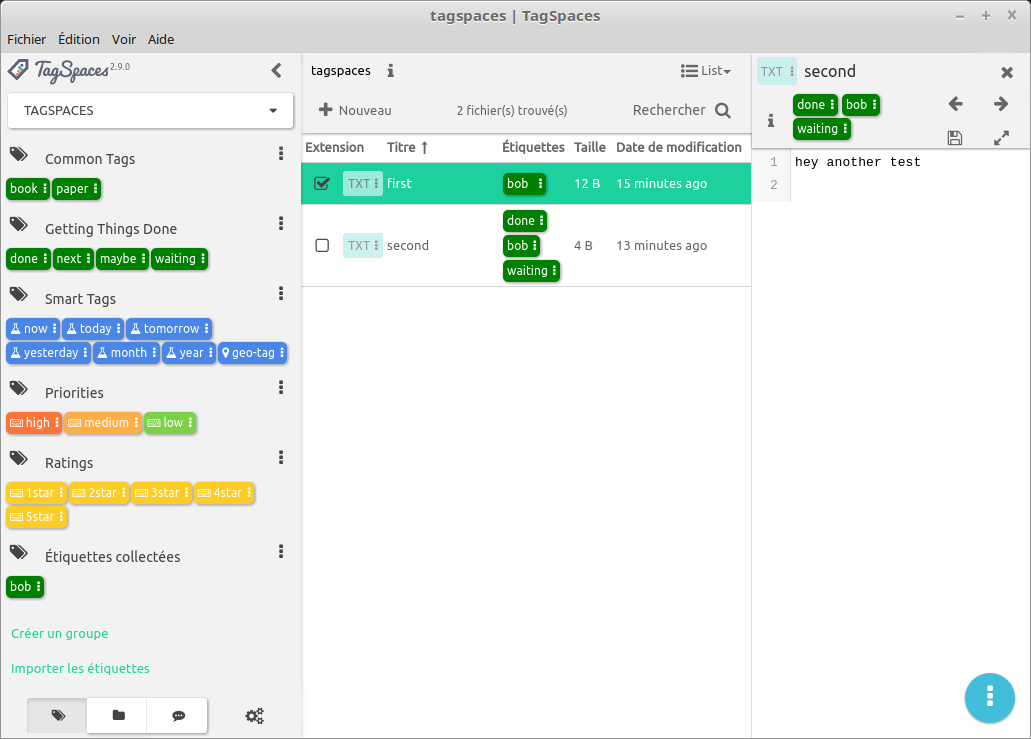
\includegraphics[width=1\textwidth]{images/tagspaces.png}
            \end{figure}
        \end{column}
        \pause
        \begin{column}{.4\textwidth}
        \fontsize{7pt}{9}\selectfont
            \begin{center}
                \begin{tabularx}{4.5cm}{|X|X|} \hline
                    \textbf{Points positifs} & \textbf{Points négatifs} \\ \hline
                    Rapide et efficace & Dépendance à une BDD externe \\ \hline
                    Open source & Modification et accès uniquement par l'application \\ \hline
                    GUI & \\ \hline
                \end{tabularx}
            \end{center}
        \end{column}
    \end{columns}
\end{frame}

\subsection{macOS}
\begin{frame}
    \frametitle{\subsecname}
    \begin{columns}[T]
        \begin{column}{.4\textwidth}
            \begin{center}
                \begin{figure}
                    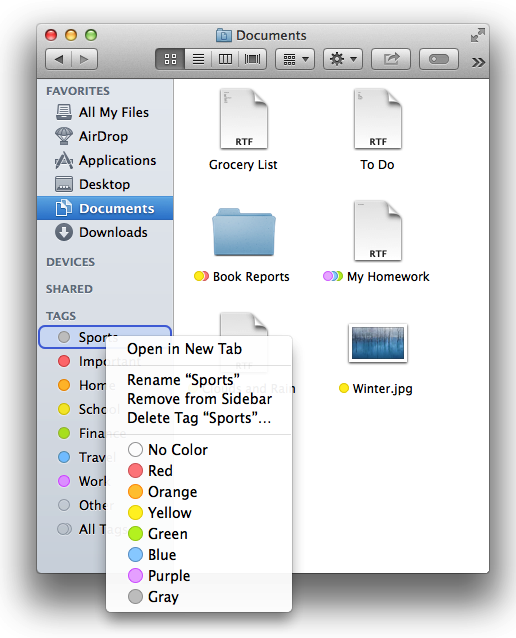
\includegraphics[width=1\textwidth]{images/macos_tags.png}
                \end{figure}
            \end{center}
        \end{column}
        \pause
        \begin{column}{.6\textwidth}
        % \fontsize{7pt}{9}\selectfont
            \begin{center}
                \begin{tabularx}{6cm}{|X|X|} \hline
                    \textbf{Points positifs} & \textbf{Points négatifs} \\ \hline
                    Système de tags intégré à l'explorateur de fichiers & Pas open source \\ \hline
                    Stocke les tags dans les attributs des fichiers & Seulement pour macOS \\ \hline
                    Performant & Non écrit en Rust \\ \hline
                \end{tabularx}
            \end{center}
        \end{column}
    \end{columns}
\end{frame}

%%%%%%%%%%%%%%%%%%%%%%%%%%%%%%%%%%%%%%%%%%%%%%%%%%%%%%%%%%%%%%%%%%%%%%%%%%%%%%%%%%%%%%%%%%%%%%%%%%
%%%%%%%%%%%%%%%%%%%%%%%%%%%%%%%%%%%%%%%%%%%%%%%%%%%%%%%%%%%%%%%%%%%%%%%%%%%%%%%%%%%%%%%%%%%%%%%%%%
\section{Architecture}
\subsection{Gestion des tags}
\begin{frame}
    \frametitle{\subsecname}
    \begin{itemize}
        \item Stockage des tags dans les attributs étendus (XATTR).
        \item Outil dédié plutôt que reprendre les commandes existantes.
        \item Confort d'utilisation.
    \end{itemize}
\end{frame}

\subsection{Indexation des fichiers et des tags}
\begin{frame}
    \frametitle{\subsecname}
    \begin{columns}[T]
        \begin{column}{.5\textwidth}
            \begin{center}
                \begin{figure}
                    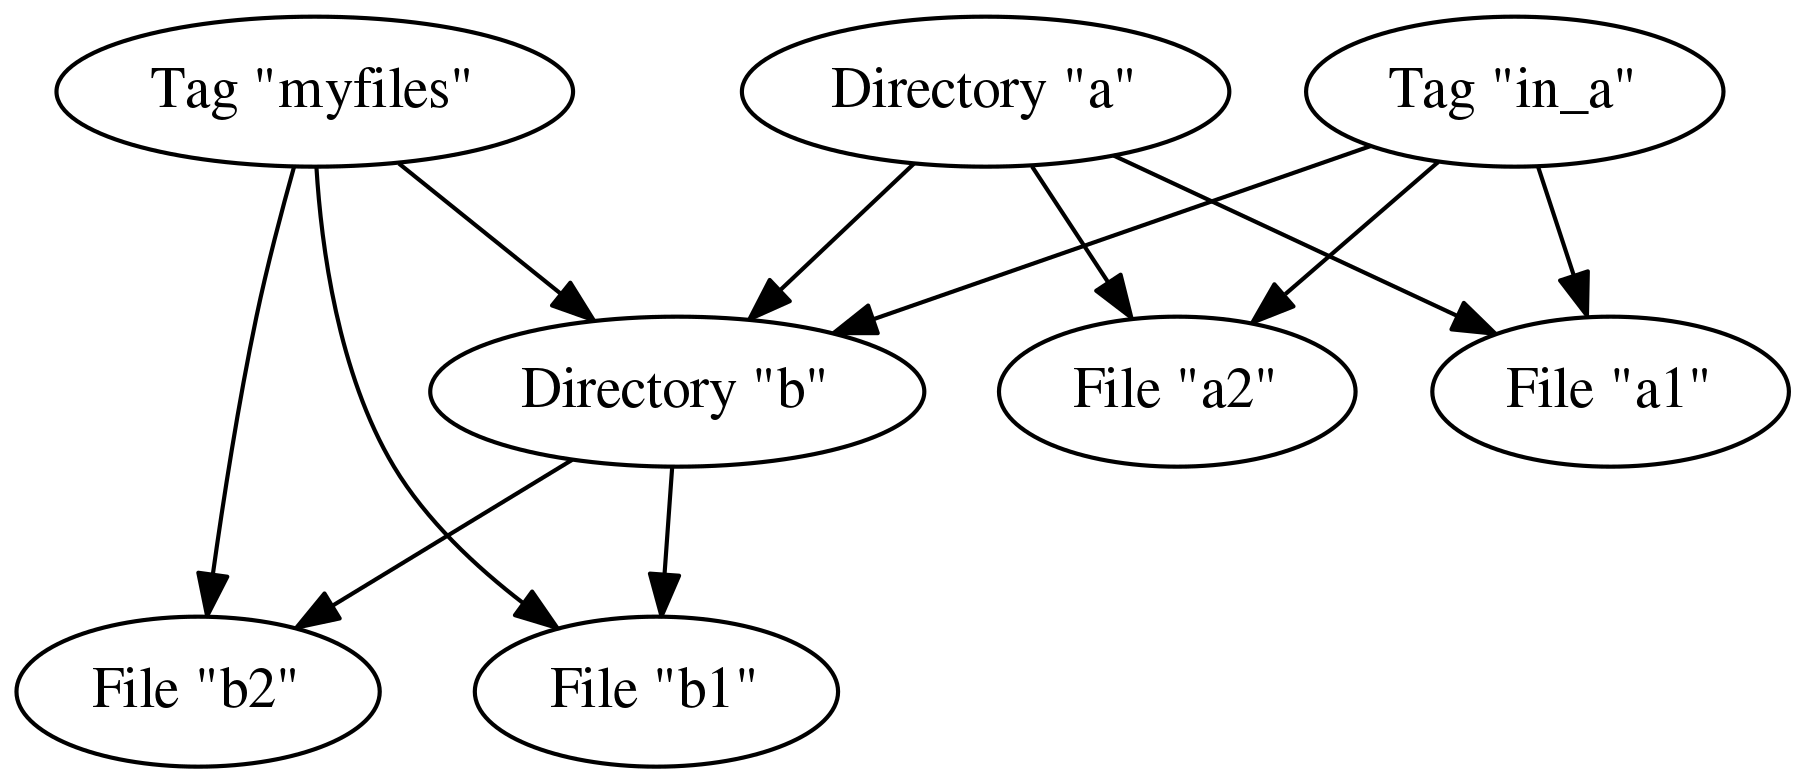
\includegraphics[width=1\textwidth]{images/graph.png}
                \end{figure}
            \end{center}
        \end{column}
        \pause
        \begin{column}{.5\textwidth}
            \begin{center}
                \begin{figure}
                    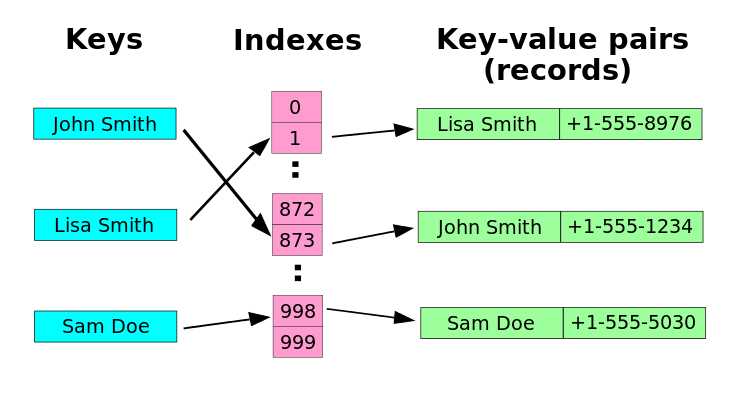
\includegraphics[width=1\textwidth]{images/hashmap_wiki.png}
                \end{figure}
            \end{center}
        \end{column}
    \end{columns}
\end{frame}

\subsection{Surveillance du système de fichiers}
\begin{frame}
    \frametitle{\subsecname}
    \begin{itemize}
        \item Mise à jour du graphe lors des événements suivants :
        \begin{itemize}
            \item Changement sur les tags.
            \item Création de fichiers/répertoires.
            \item Suppression de fichiers/répertoires.
            \item Déplacement/renommage de fichiers/répertoires.
        \end{itemize}
        \item Pattern producer-consumer.
    \end{itemize}
\end{frame}

\subsection{Requêtes de tags et fichiers}
\begin{frame}
    \frametitle{\subsecname}
    \begin{itemize}
        \item Lister les fichiers et répertoires associés à des tags (expressions logiques).
        \item Lister les tags existants.
        \item Renommer un tag.
    \end{itemize}
\end{frame}

%%%%%%%%%%%%%%%%%%%%%%%%%%%%%%%%%%%%%%%%%%%%%%%%%%%%%%%%%%%%%%%%%%%%%%%%%%%%%%%%%%%%%%%%%%%%%%%%%%%
%%%%%%%%%%%%%%%%%%%%%%%%%%%%%%%%%%%%%%%%%%%%%%%%%%%%%%%%%%%%%%%%%%%%%%%%%%%%%%%%%%%%%%%%%%%%%%%%%%%
\section{Technologies}
\subsection{Rust}
\subsubsection{Généralités}
\begin{frame}[fragile]
    \frametitle{\subsecname}
    \framesubtitle{Généralités (1)}
    \begin{itemize}
        \item Langage moderne, performant, fiable, compilé, et fortement typé.
        \item Disponible sur Linux, Windows et macOS.
        \item Cargo : système de compilation et d'exécution et gestionnaire de paquets intégré à Rust.
        \item Structures, collections, énumérations et pattern matching. 
    \end{itemize}

    \begin{minted}[bgcolor=mygray,breaklines,breaksymbol=,linenos,frame=single,stepnumber=1,tabsize=2]{rust}
enum Direction { North, South, East, West }
match direction {
  Direction::North => println!("Go North"),
  Direction::South => println!("Go South"),
  _ => println!("Go East or West") //clause par défaut
}
    \end{minted}
\end{frame}

\begin{frame}[fragile]
    \frametitle{\subsecname}
    \framesubtitle{Généralités (2)}
    \begin{itemize}
        \item Tests.
        \item Gestion des erreurs.
    \end{itemize}
    \begin{minted}[bgcolor=mygray,breaklines,breaksymbol=,linenos,frame=single,stepnumber=1,tabsize=2]{rust}
enum Result<T, E> { Ok(T), Err(E), }
match value {
  Ok(data) => println!("u32 value : {}", data),
  Err(error) => println!("Error : {}", error)
}
    \end{minted}
\end{frame}

\begin{frame}
    \frametitle{\subsecname}
    \framesubtitle{Généralités (3)}
    \begin{itemize}
        \item Unsafe Rust.
        \item Concurrence et Threads.
    \end{itemize}
    \begin{center}
        \begin{figure}
            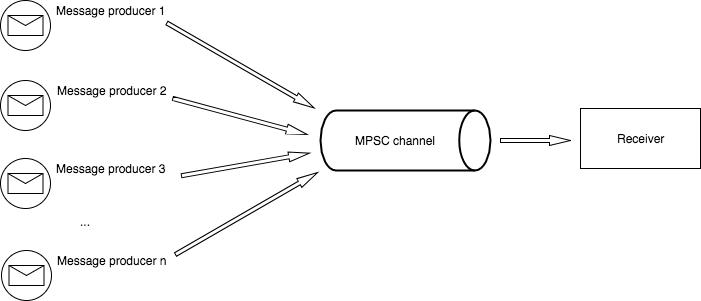
\includegraphics[width=0.8\textwidth]{images/mpsc.png}
        \end{figure}
    \end{center}
\end{frame}

\subsubsection{Ownership et Borrowing}
\begin{frame}
    \frametitle{\subsecname}
    \framesubtitle{Ownership et Borrowing (1)}
    \textbf{Ownership}
    \begin{itemize}
        \item Chaque variable est dite le "possesseur" (\textit{owner}) d'une valeur.
        \item Il ne peut y avoir qu'un seul \textit{owner} pour une valeur.
        \item Lorsque l'\textit{owner} est détruit ou change de portée, la valeur est détruite.
    \end{itemize}
    \bigbreak
    \textbf{Borrowing}
    \begin{enumerate}
        \item À tout moment, il ne peut y avoir soit une seule référence mutable, soit plusieurs 
            références immutables, mais pas les deux en même temps.
        \item Les références doivent toujours être valides.
    \end{enumerate}
\end{frame}

\begin{frame}[fragile]
    \frametitle{\subsecname}
    \framesubtitle{Ownership et Borrowing (2)}
    \begin{minted}[bgcolor=mygray,breaklines,breaksymbol=,linenos,frame=single,stepnumber=1,tabsize=2]{rust}
let a = 10;
let b = a;
let mut my_vec = vec![3, 2, 1]; 
let other_vec = my_vec;
my_vec.push(42); // Erreur, la valeur a été déplacée
    \end{minted}
    \begin{minted}[bgcolor=mygray,breaklines,breaksymbol=,linenos,frame=single,stepnumber=1,tabsize=2]{rust}
fn main() {
    let mut my_vec = vec![3, 2, 1];
    ref_immutable(&my_vec);
    ref_mutable(&mut my_vec);
}
fn ref_immutable(v : &Vec<i32>) { println!("{:?}", v); }
fn ref_mutable(v : &mut Vec<i32>) { v.push(42); }
    \end{minted}
\end{frame}

\subsection{Attributs étendus (XATTR)}
\begin{frame}
    \frametitle{\subsecname}
    \begin{itemize}
        \item Métadonnées sous forme de paire \mintinline{text}{espace.nom:valeur}.
        \item Nom = chaine de caractères, valeur = chaine de caractères ou données binaires.
        \item Existent sous ext2-3-4, XFS, Btrfs, UFS1-2, NTFS, HFS+, ZFS.
    \end{itemize}
\end{frame}

\subsection{Inotify}
\begin{frame}
    \frametitle{\subsecname}
    \begin{itemize}
        \item API de notifications d'événements sur le système de fichiers.
        \item Trois appels système : initialisation, ajout de surveillance sur un chemin de fichiers 
            donné et suppression de cette surveillance.
        \item Lecture d'un événement avec read().
    \end{itemize}
\end{frame}

\subsection{Sockets}
\begin{frame}
    \frametitle{\subsecname}
    \begin{center}
        \begin{figure}
            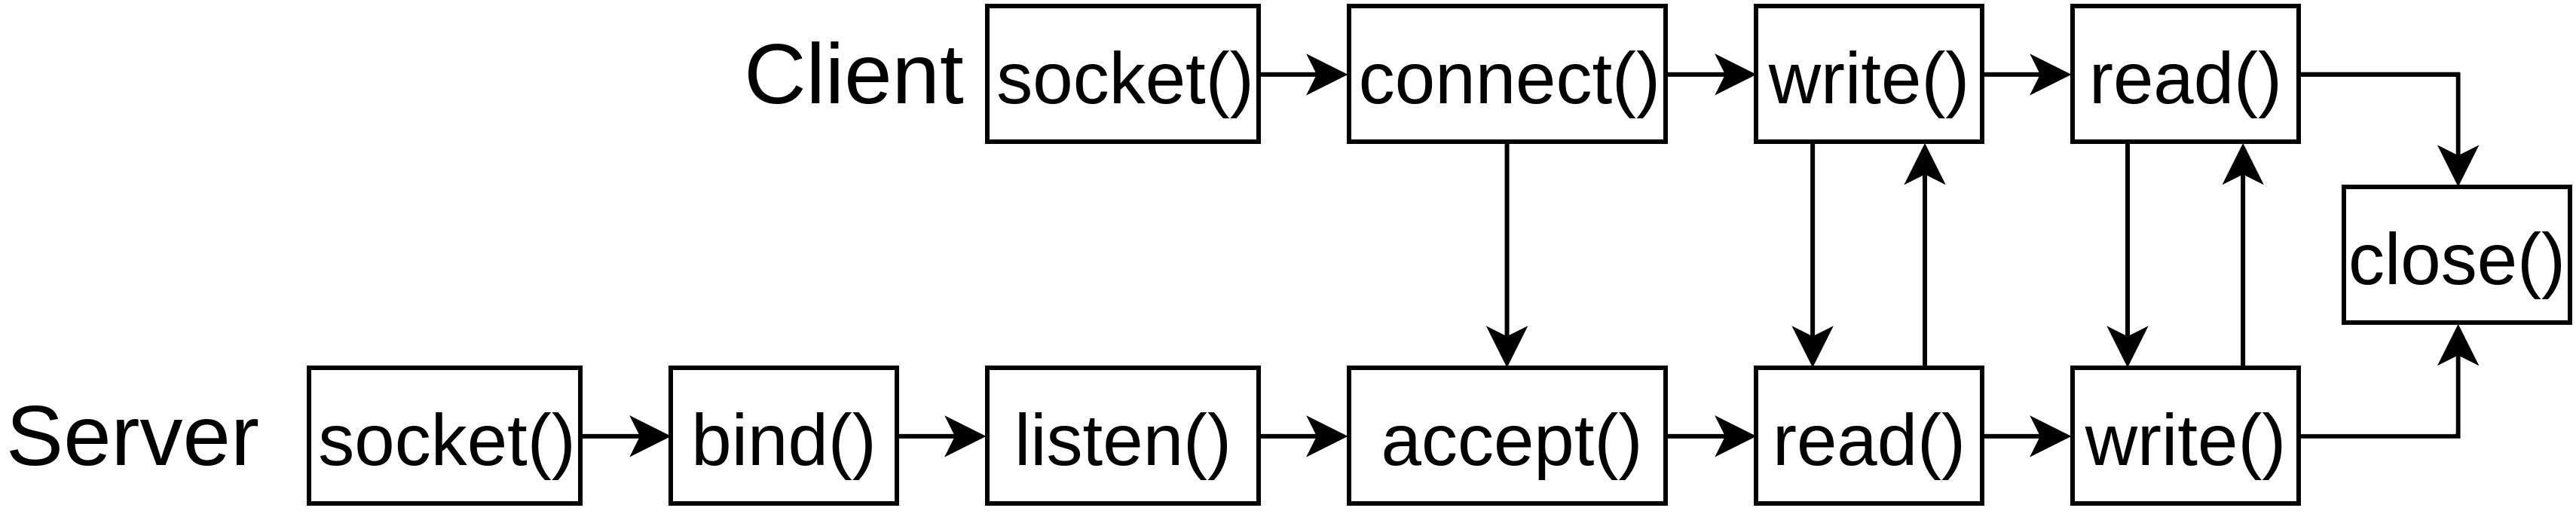
\includegraphics[width=1\textwidth]{images/sockets2.png}
        \end{figure}
    \end{center}
\end{frame}

%%%%%%%%%%%%%%%%%%%%%%%%%%%%%%%%%%%%%%%%%%%%%%%%%%%%%%%%%%%%%%%%%%%%%%%%%%%%%%%%%%%%%%%%%%%%%%%%%%%
%%%%%%%%%%%%%%%%%%%%%%%%%%%%%%%%%%%%%%%%%%%%%%%%%%%%%%%%%%%%%%%%%%%%%%%%%%%%%%%%%%%%%%%%%%%%%%%%%%%
\section{Réalisation}
\subsection{Tag Manager}
\begin{frame}
    \frametitle{\subsecname}
    \begin{columns}[T]
        \begin{column}{.5\textwidth}
            \begin{center}
                \begin{figure}
                    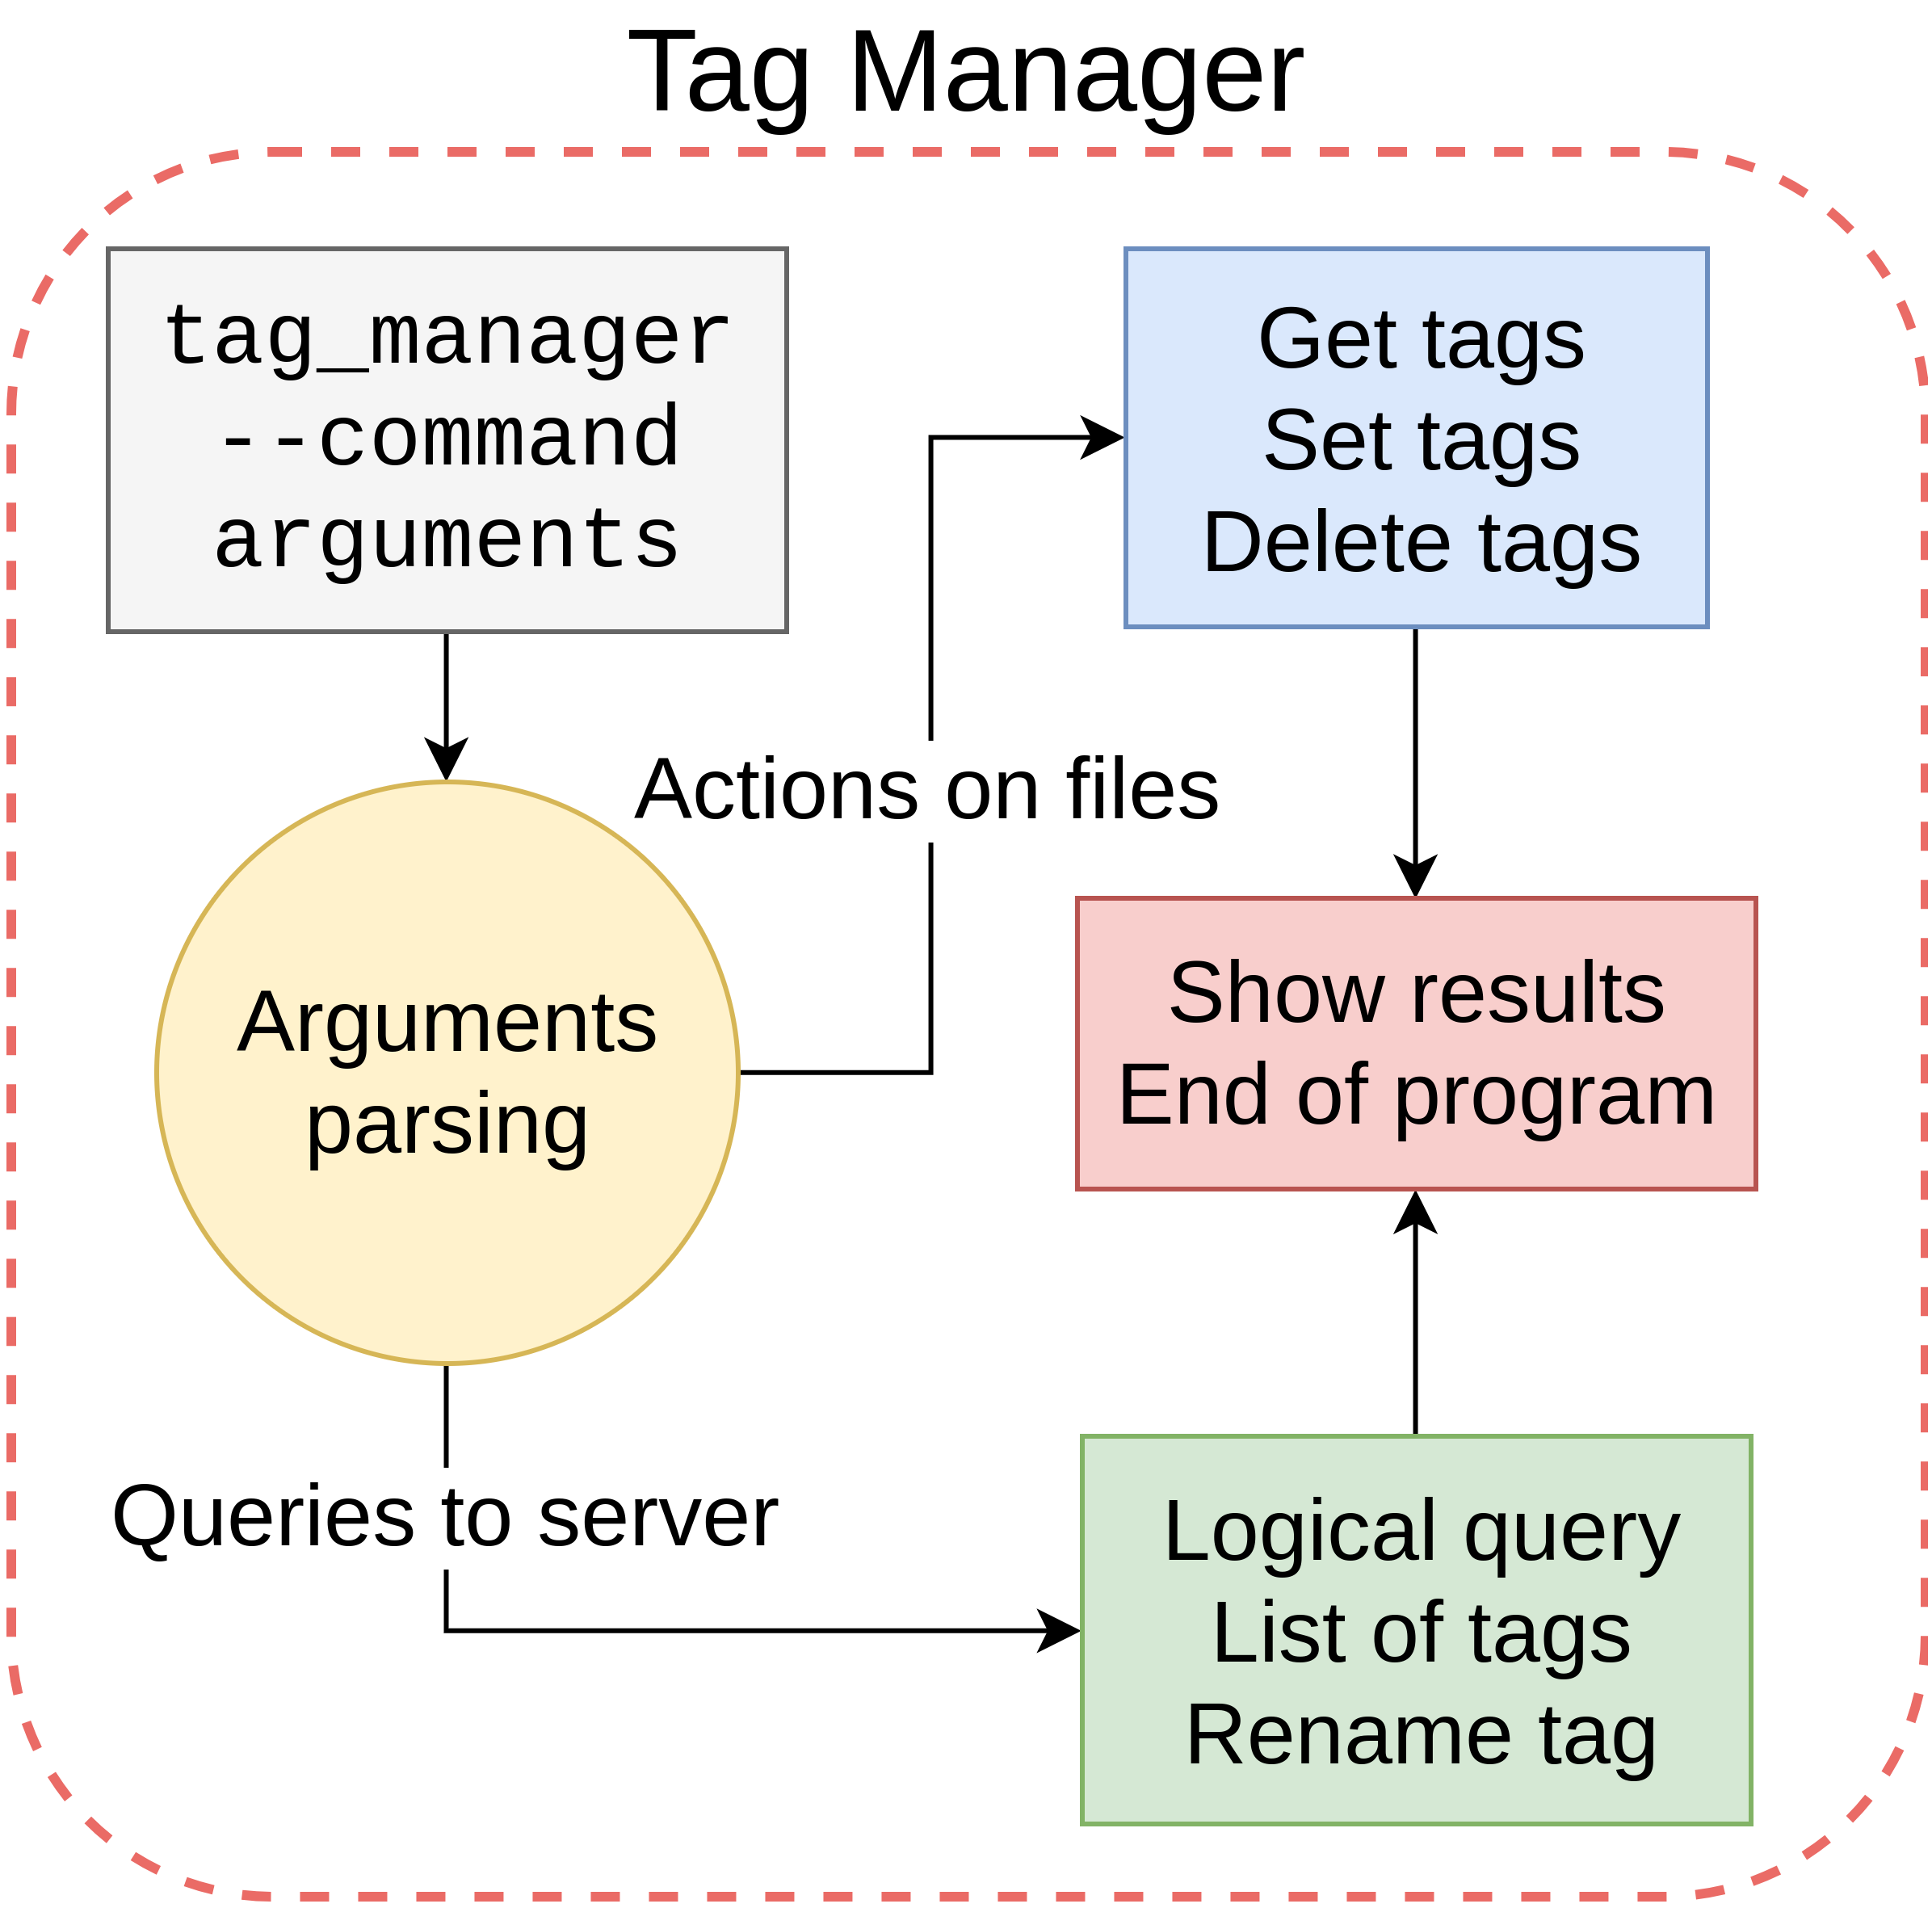
\includegraphics[width=1\textwidth]{images/tag_manager2.png}
                \end{figure}
            \end{center}
        \end{column}
        \pause
        \begin{column}{.5\textwidth}
            \begin{itemize}
                \item CLI.
                \item Gestion des tags.
                \item Requêtes sur les tags et fichiers.
                \item Manipule les XATTR des fichiers.
                \item Programme "client".
            \end{itemize}
        \end{column}
    \end{columns}
\end{frame}

\subsection{Tag Engine}
\begin{frame}
    \frametitle{\subsecname}
    \begin{columns}[T]
        \begin{column}{.5\textwidth}
            \begin{center}
                \begin{figure}
                    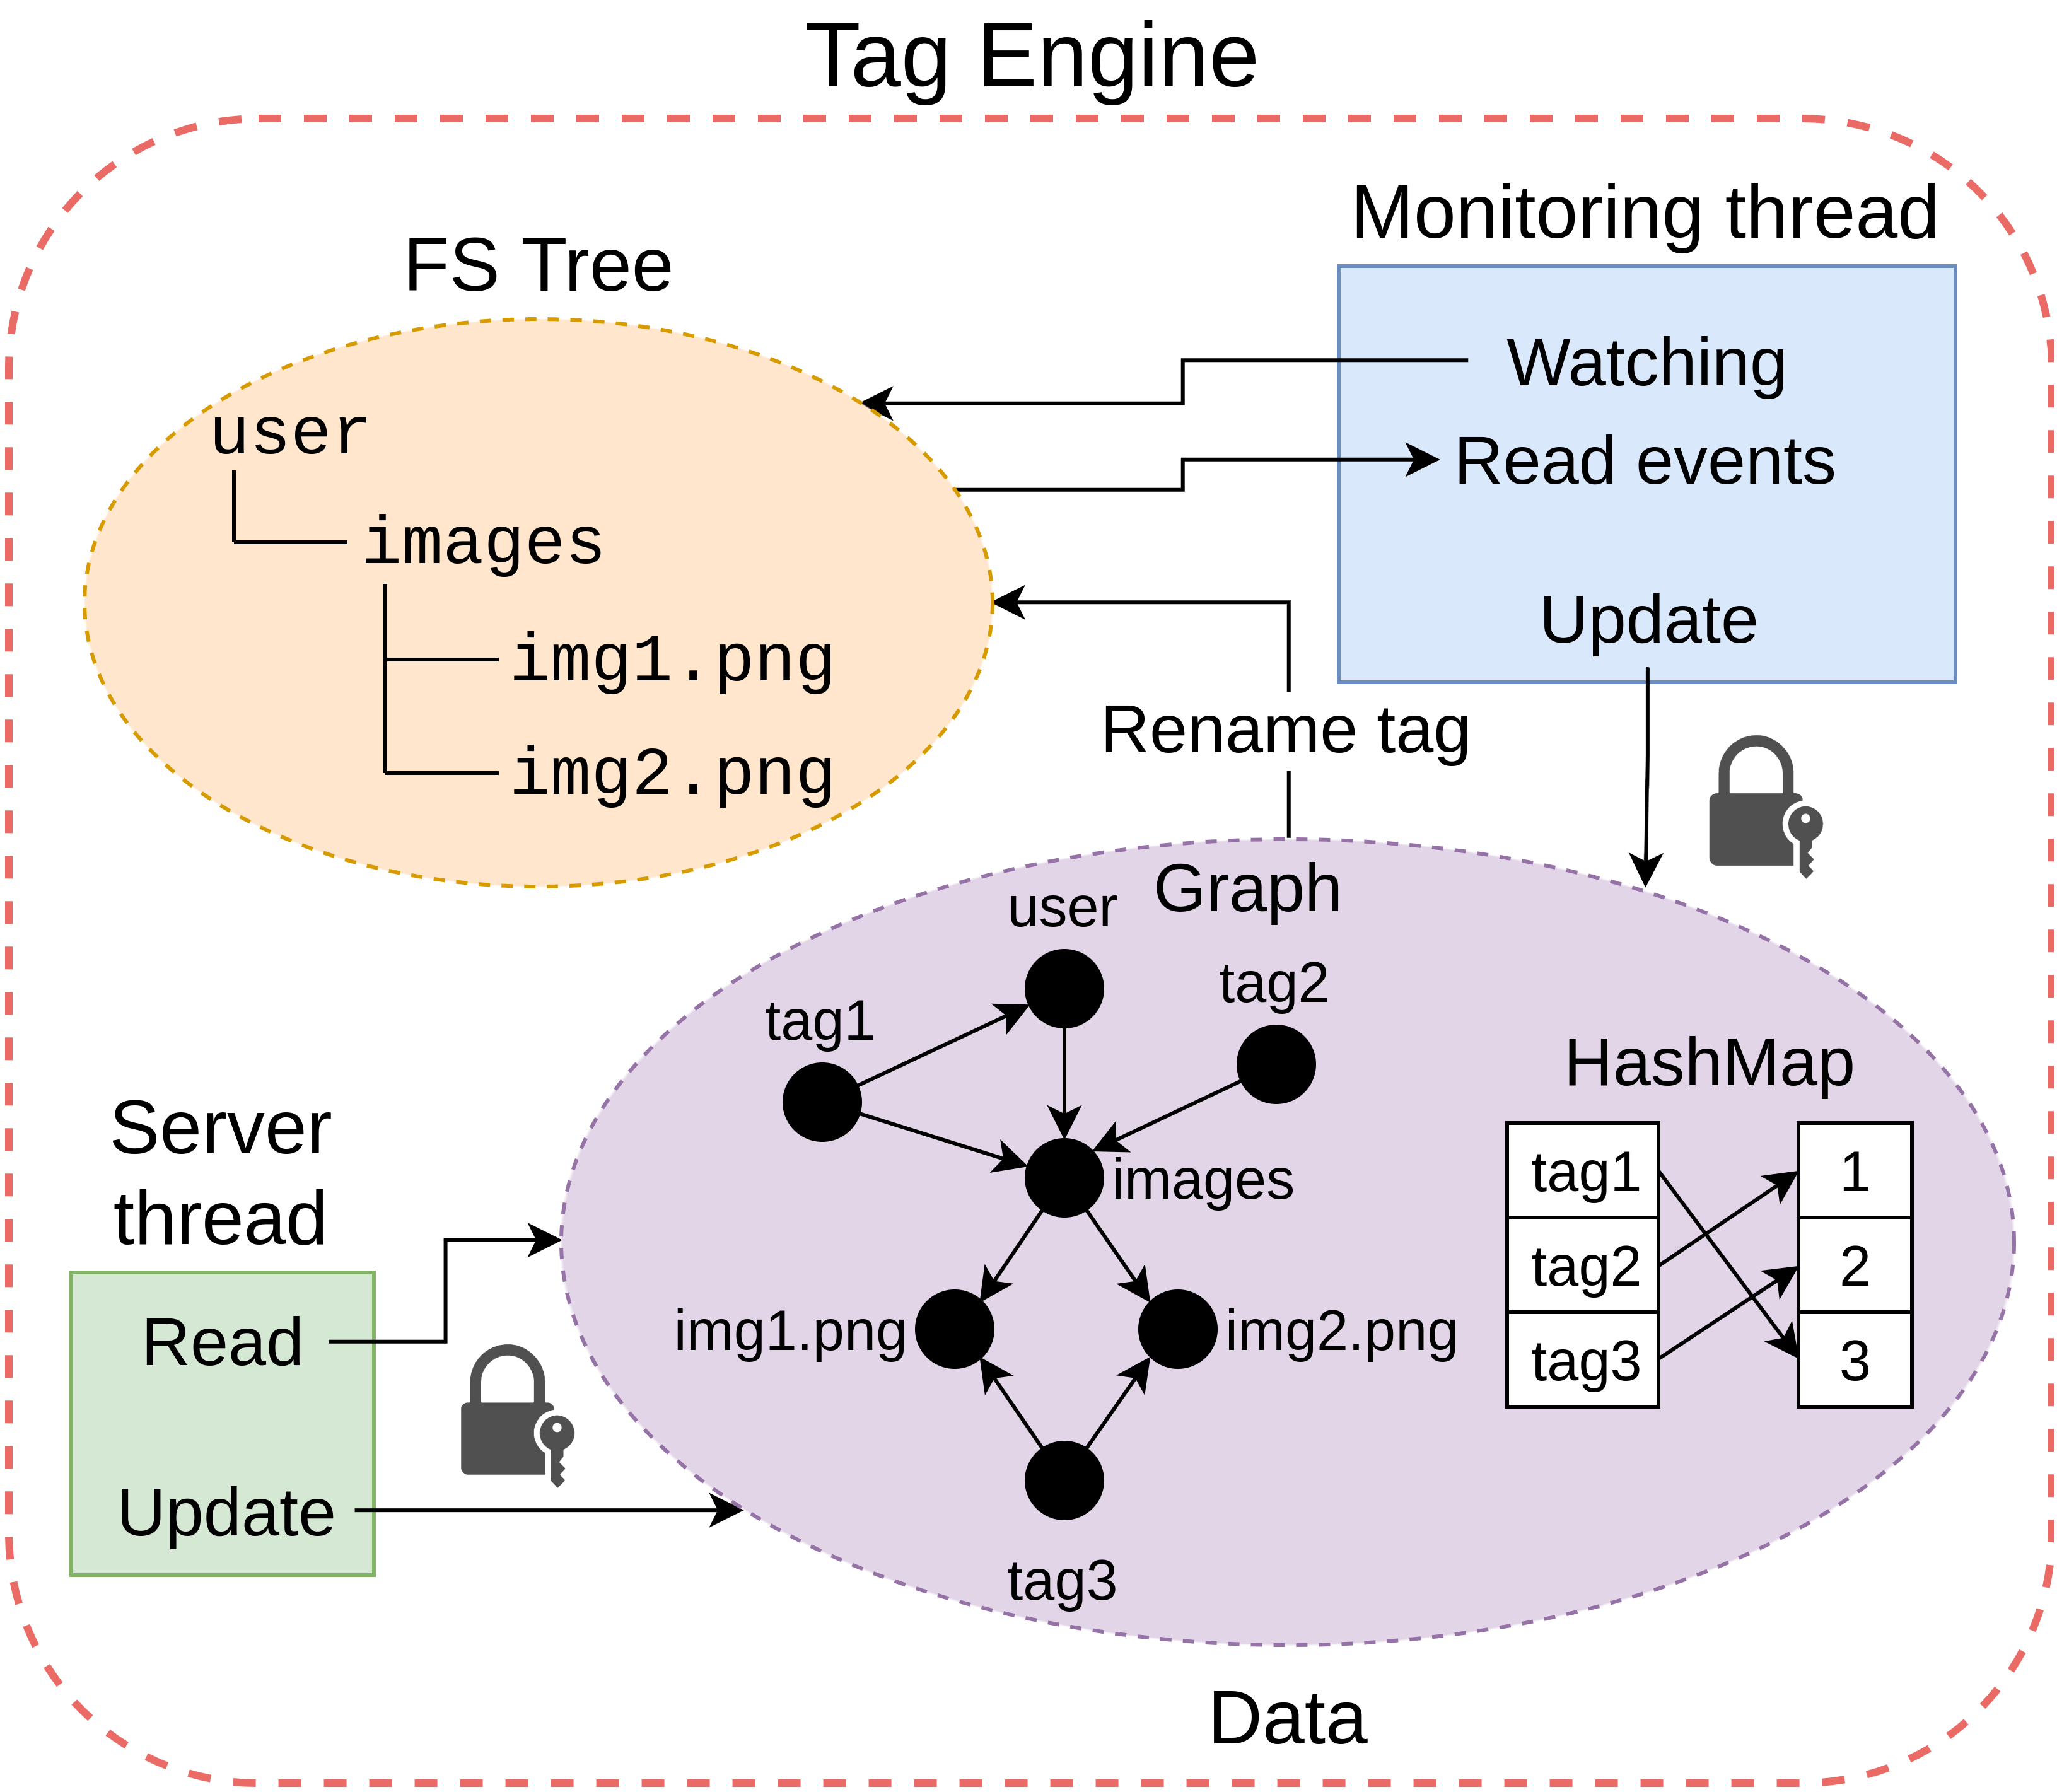
\includegraphics[width=1\textwidth]{images/tag_engine2.png}
                \end{figure}
            \end{center}
        \end{column}
        \pause
        \begin{column}{.5\textwidth}
            \begin{itemize}
                \item Surveille l'arborescence des fichiers.
                \item Écoute sur une socket les requêtes provenant de Tag Manager.
                \item Maintient la relation entre tags, fichiers et répertoires à l'aide d'un graphe orienté et d'une hashmap.
                \item Les changements sur le FS sont répercutés sur le graphe.
                \item Multithread.
            \end{itemize}
        \end{column}
    \end{columns}
\end{frame}

\subsection{TagFS}
\begin{frame}
    \frametitle{\subsecname}
    \begin{center}
        \begin{figure}
            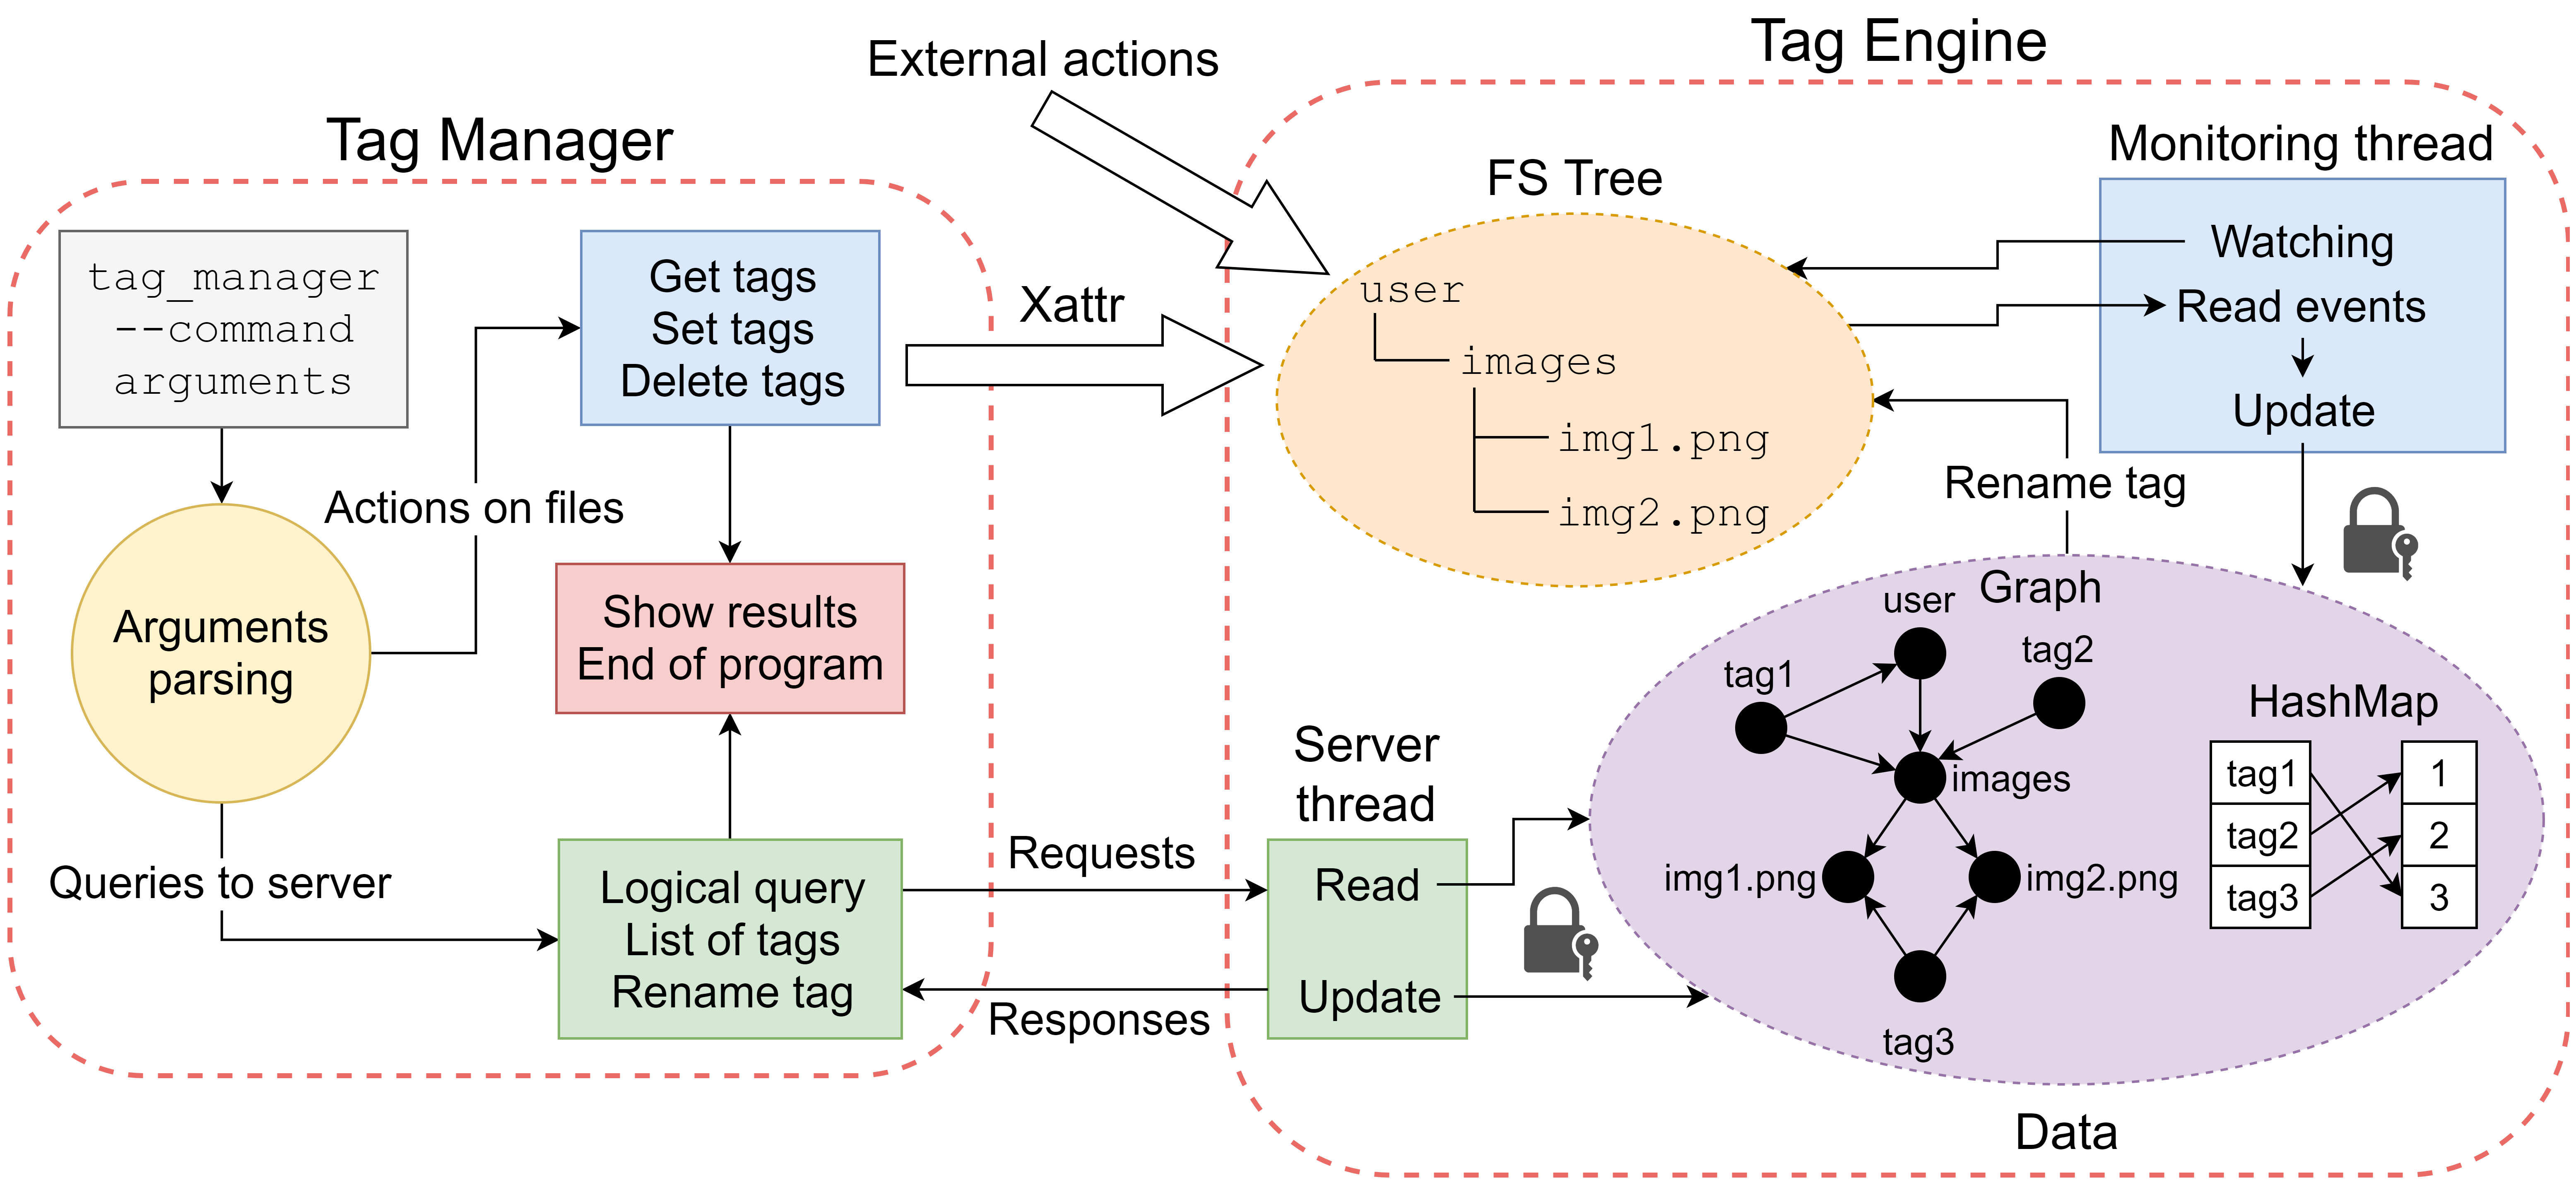
\includegraphics[width=1\textwidth]{images/tagfs4.png}
        \end{figure}
    \end{center}
\end{frame}

\subsection{Démo}
\begin{frame}
    \frametitle{\subsecname}
    % TODO: vidéo
\end{frame}

%%%%%%%%%%%%%%%%%%%%%%%%%%%%%%%%%%%%%%%%%%%%%%%%%%%%%%%%%%%%%%%%%%%%%%%%%%%%%%%%%%%%%%%%%%%%%%%%%%%
%%%%%%%%%%%%%%%%%%%%%%%%%%%%%%%%%%%%%%%%%%%%%%%%%%%%%%%%%%%%%%%%%%%%%%%%%%%%%%%%%%%%%%%%%%%%%%%%%%%
\section{Discussion}
\subsection{Mesures de performances}
\begin{frame}
    \frametitle{\subsecname}
    \begin{columns}[T]
        \begin{column}{.35\textwidth}
        \fontsize{6pt}{8}\selectfont
            \begin{tabularx}{4cm}{|p{1cm}|p{1cm}|X|} \hline
                \textbf{Répertoire} & \textbf{Sous-répertoires} & \textbf{Fichiers} \\ \hline
                Android & 15'172 & 112'046 \\ \hline
                android-studio & 3'331 & 13'287 \\ \hline
                bin & 553 & 9'306 \\ \hline
                Documents & 15'442 & 64'486 \\ \hline
                Dropbox & 2'377 & 8'659 \\ \hline
                Images & 5 & 863 \\ \hline
                Musique & 135 & 1'352 \\ \hline
            \end{tabularx}
        \end{column}
        \pause
        \begin{column}{.65\textwidth}
            \begin{center}
                \begin{figure}
                    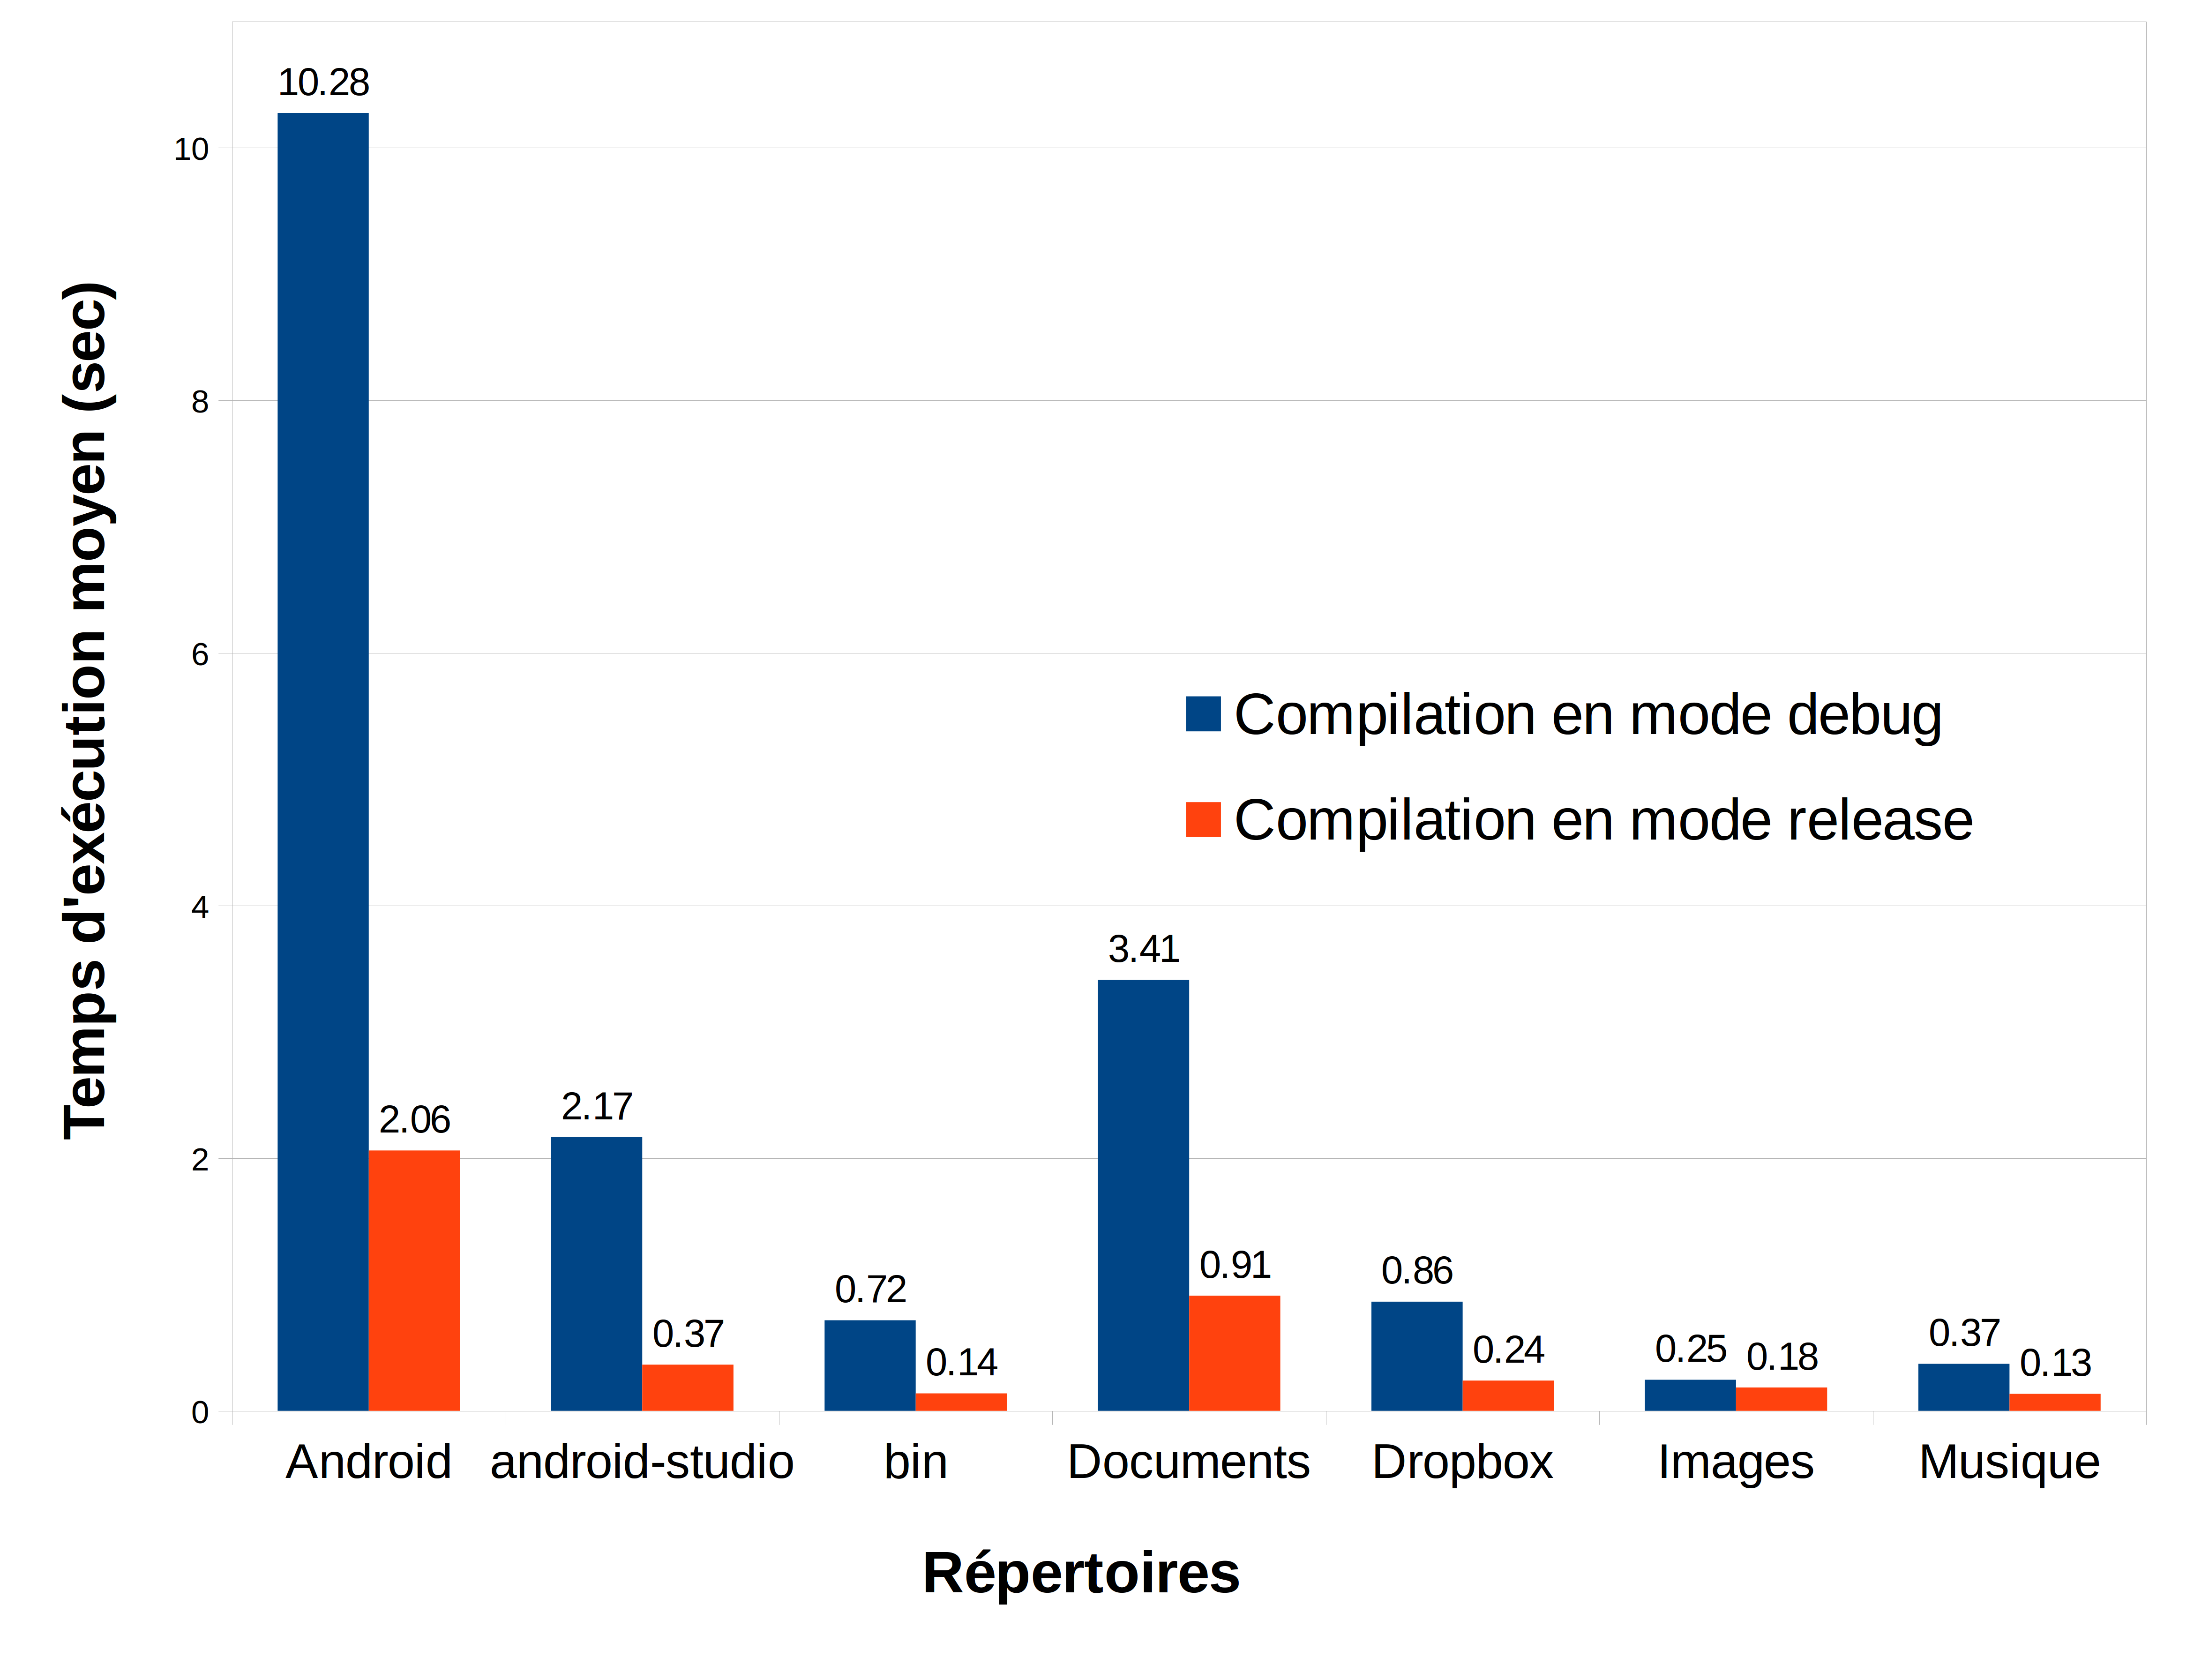
\includegraphics[width=1\textwidth]{images/histo.png}
                \end{figure}
            \end{center}
        \end{column}
    \end{columns}
\end{frame}

\subsection{Rust vs C}
\begin{frame}
    \frametitle{\subsecname}
    \begin{center}
        \begin{tabularx}{11cm}{|X|X|} \hline
            \textbf{Avantages par rapport à C} & \textbf{Inconvénients par rapport à C} \\ \hline
            Garanties sécurité mémoire & Courbe d'apprentissage plus longue \\ \hline
            Détection des erreurs à la compilation & Contraintes du langage parfois handicapantes \\ \hline
            Compilateur verbeux & Moins répandu \\ \hline
            Performances égales ou très proches & Manque de soutien global \\ \hline
            Gestion des erreurs &  \\ \hline
            Absence de NULL &  \\ \hline
            Cargo et Crates.io &  \\ \hline
            Librairie standard &  \\ \hline
            Généricité &  \\ \hline
        \end{tabularx}
    \end{center}
\end{frame}

%%%%%%%%%%%%%%%%%%%%%%%%%%%%%%%%%%%%%%%%%%%%%%%%%%%%%%%%%%%%%%%%%%%%%%%%%%%%%%%%%%%%%%%%%%%%%%%%%%%
%%%%%%%%%%%%%%%%%%%%%%%%%%%%%%%%%%%%%%%%%%%%%%%%%%%%%%%%%%%%%%%%%%%%%%%%%%%%%%%%%%%%%%%%%%%%%%%%%%%
\section{Conclusion}
\begin{frame}
    \frametitle{\secname}
    % TODO: conclusion
    \begin{itemize}
        \item 
    \end{itemize}
\end{frame}

%%%%%%%%%%%%%%%%%%%%%%%%%%%%%%%%%%%%%%%%%%%%%%%%%%%%%%%%%%%%%%%%%%%%%%%%%%%%%%%%%%%%%%%%%%%%%%%%%%%
%%%%%%%%%%%%%%%%%%%%%%%%%%%%%%%%%%%%%%%%%%%%%%%%%%%%%%%%%%%%%%%%%%%%%%%%%%%%%%%%%%%%%%%%%%%%%%%%%%%
% \section*{Remerciements}
\begin{frame}
    \frametitle{Remerciements}
    % TODO: références
\end{frame}

%%%%%%%%%%%%%%%%%%%%%%%%%%%%%%%%%%%%%%%%%%%%%%%%%%%%%%%%%%%%%%%%%%%%%%%%%%%%%%%%%%%%%%%%%%%%%%%%%%%
%%%%%%%%%%%%%%%%%%%%%%%%%%%%%%%%%%%%%%%%%%%%%%%%%%%%%%%%%%%%%%%%%%%%%%%%%%%%%%%%%%%%%%%%%%%%%%%%%%%
% \section*{Références}
\begin{frame}
    \frametitle{Références}
    % TODO: références
\end{frame}


\end{document}
